%% LyX 2.1.3 created this file.  For more info, see http://www.lyx.org/.
%% Do not edit unless you really know what you are doing.
\documentclass{article}\usepackage[]{graphicx}\usepackage[]{color}
%% maxwidth is the original width if it is less than linewidth
%% otherwise use linewidth (to make sure the graphics do not exceed the margin)
\makeatletter
\def\maxwidth{ %
  \ifdim\Gin@nat@width>\linewidth
    \linewidth
  \else
    \Gin@nat@width
  \fi
}
\makeatother

\definecolor{fgcolor}{rgb}{0.345, 0.345, 0.345}
\newcommand{\hlnum}[1]{\textcolor[rgb]{0.686,0.059,0.569}{#1}}%
\newcommand{\hlstr}[1]{\textcolor[rgb]{0.192,0.494,0.8}{#1}}%
\newcommand{\hlcom}[1]{\textcolor[rgb]{0.678,0.584,0.686}{\textit{#1}}}%
\newcommand{\hlopt}[1]{\textcolor[rgb]{0,0,0}{#1}}%
\newcommand{\hlstd}[1]{\textcolor[rgb]{0.345,0.345,0.345}{#1}}%
\newcommand{\hlkwa}[1]{\textcolor[rgb]{0.161,0.373,0.58}{\textbf{#1}}}%
\newcommand{\hlkwb}[1]{\textcolor[rgb]{0.69,0.353,0.396}{#1}}%
\newcommand{\hlkwc}[1]{\textcolor[rgb]{0.333,0.667,0.333}{#1}}%
\newcommand{\hlkwd}[1]{\textcolor[rgb]{0.737,0.353,0.396}{\textbf{#1}}}%

\usepackage{framed}
\makeatletter
\newenvironment{kframe}{%
 \def\at@end@of@kframe{}%
 \ifinner\ifhmode%
  \def\at@end@of@kframe{\end{minipage}}%
  \begin{minipage}{\columnwidth}%
 \fi\fi%
 \def\FrameCommand##1{\hskip\@totalleftmargin \hskip-\fboxsep
 \colorbox{shadecolor}{##1}\hskip-\fboxsep
     % There is no \\@totalrightmargin, so:
     \hskip-\linewidth \hskip-\@totalleftmargin \hskip\columnwidth}%
 \MakeFramed {\advance\hsize-\width
   \@totalleftmargin\z@ \linewidth\hsize
   \@setminipage}}%
 {\par\unskip\endMakeFramed%
 \at@end@of@kframe}
\makeatother

\definecolor{shadecolor}{rgb}{.97, .97, .97}
\definecolor{messagecolor}{rgb}{0, 0, 0}
\definecolor{warningcolor}{rgb}{1, 0, 1}
\definecolor{errorcolor}{rgb}{1, 0, 0}
\newenvironment{knitrout}{}{} % an empty environment to be redefined in TeX

\usepackage{alltt} 
\usepackage{ucs}
\usepackage[utf8x]{inputenc}
\usepackage[sc]{mathpazo}
\usepackage[T1]{fontenc}
\usepackage{geometry}

\newenvironment{uzdevums}[1][\unskip]{%
\vspace{3mm}
\noindent
\textbf{#1 uzdevums:}
\noindent}
{}

\geometry{verbose,tmargin=2.5cm,bmargin=2.5cm,lmargin=2.5cm,rmargin=2.5cm}
\setcounter{secnumdepth}{2}
\setcounter{tocdepth}{2}
\usepackage{url}
\usepackage[unicode=true,pdfusetitle,
 bookmarks=true,bookmarksnumbered=true,bookmarksopen=true,bookmarksopenlevel=2,
 breaklinks=false,pdfborder={0 0 1},backref=false,colorlinks=false]
 {hyperref}
\renewcommand{\abstractname}{Anotācija}
\hypersetup{
 pdfstartview={XYZ null null 1}}
\IfFileExists{upquote.sty}{\usepackage{upquote}}{}
\begin{document}



\title{41.\ AMO rezultāti tabulās un zīmējumos}

\author{}
\date{}

\maketitle

\begin{abstract}
Šajā dokumentā apkopoti daži 41.\ Atklātās matemātikas olimpiādes (2014.m.g.) rezultātu kop\-sa\-vil\-ku\-mi. Izmantojot izklājlapas, ko publisko LU Neklātienes Matemātikas Skola, aprēķināts dalībnieku skaits, dalības aktivitāte (AMO dalībnieku īpatsvars no visiem attiecīgā vecuma skolēniem), dalība un rezultāti atkarībā no skolēnu \v{g}eogrāfijas, urbanizācijas, valodas, dzimuma. Apkopoti saraksti ar skolotājiem un skolām, kas nodrošinājuši augstu dalību vai ieguvuši lielu punktu kopskaitu. Pārskata nobeigumā minēti dati arī par uzdevumiem --- vidējais punktu skaits un vērtējumu sadalījums, kāda daļa no rēķinātājiem neuzsāka risināt (``mīnusu'' jeb neatrasto risinājumu skaits galavērtējumā), kāda ir konkrētā uzdevuma vērtējumu korelācija ar pārējo uzdevumu vērtējumu summu. 
\end{abstract}

\section{Dalībnieku aktivitāte}

Šajā sadaļā atbildēsim uz jautājumu, kāda daļa no 6.klasei atbilstošās vecuma grupas skolēniem piedalījās 41.\ AMO. 
Dati par skolēnu skaitu pa re\v{g}ioniem, klasēm un mācību valodām ņemti no IZM publiskotās statistikas --- \url{http://izm.gov.lv/lv/publikacijas-un-statistika/statistika-par-visparejo-izglitibu/2014-2015-m-g}. Dati apkopoti par 9 lielajām pilsētām kā arī par re\v{g}ioniem, kuros nav ietvertas lielās pilsētas. Ar {\em re\v{g}ioniem} domāti NUTS 3 re\v{g}ioni --- sk. \url{http://en.wikipedia.org/wiki/Statistical_regions_of_Latvia} - Kurzeme, Latgale, Pierīga Rīga, Vidzeme, Zemgale.


\subsection{Dalība olimpiādē}



%% col1 = region
%% col2 = participants
%% col3 = total guys
%% col4 = percentage participated

\begin{knitrout}
\definecolor{shadecolor}{rgb}{0.969, 0.969, 0.969}\color{fgcolor}
\begin{tabular}{l|r|r|r}
\hline
  & Participants & All (Grades 5-12) & Activity \%\\
\hline
Liepaja & 48 & 4863 & 0.99\\
\hline
Ventspils & 46 & 2456 & 1.87\\
\hline
Cita Kurzeme & 95 & 9371 & 1.01\\
\hline
Daugavpils & 150 & 5206 & 2.88\\
\hline
Rezekne & 35 & 2453 & 1.43\\
\hline
Cita Latgale & 133 & 10590 & 1.26\\
\hline
Jurmala & 35 & 2507 & 1.40\\
\hline
Cita Pieriga & 376 & 15769 & 2.38\\
\hline
Riga & 1075 & 38631 & 2.78\\
\hline
Valmiera & 95 & 2275 & 4.18\\
\hline
Cita Vidzeme & 272 & 10987 & 2.48\\
\hline
Jekabpils & 44 & 1465 & 3.00\\
\hline
Jelgava & 184 & 3689 & 4.99\\
\hline
Cita Zemgale & 91 & 9739 & 0.93\\
\hline
*** Visa Latvija & 2679 & 120001 & 2.23\\
\hline
\end{tabular}


\end{knitrout}



\begin{knitrout}
\definecolor{shadecolor}{rgb}{0.969, 0.969, 0.969}\color{fgcolor}

{\centering 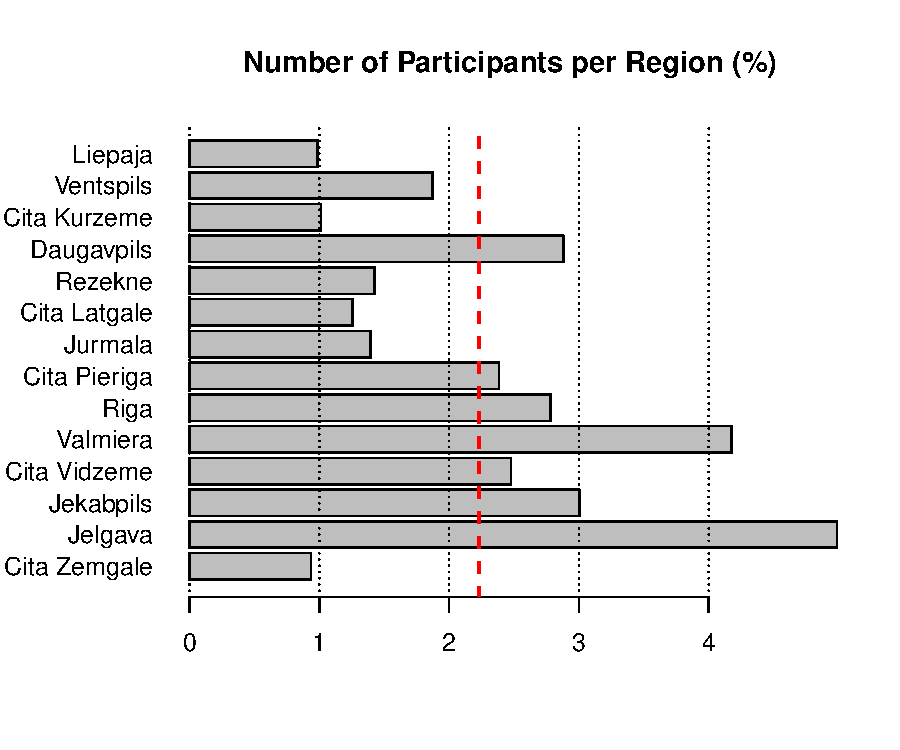
\includegraphics[width=\maxwidth]{figure/minimal-regional-activity-1} 

}



\end{knitrout}


Ir svarīgs ne tikai dalībnieku skaits, bet arī viņu sagatavotības līmenis. Šajā grafikā ikviena olimpiādes dalībnieka rezultātam ir aprēķināta z-normalizētā vērtība jeb {\em z-score}, t.i. no iegūtā punktu skaita jeb {\em raw score} atņem attiecīgās klases aritmētisko vidējo un izdala ar attiecīgās klases standartnovirzi. Pēc tam katrā re\v{g}ionā un katrā klašu grupā atsevišķi rēķina šo z-normalizēto vērtību aritmētisko vidējo. Kā redzams diagrammā, vislabākie vērtējumi olimpiādēs ir Latgalē (zilais grafiks) un Rīgā (sarkanais grafiks). Jaunāko klašu grupās Latgales skolnieku rezultāti pārsniedz valstī vidējo par aptuveni 0.3-0.5 standartnovirzēm. (Tipiski jebkurā klašu grupā punktu skaita standartnovirze ir $\sigma \in [8,11]$, t.i. Latgales skolēnu rezultāti vidēji ir par 3-4 punktiem augstāki nekā citur. Tomēr salīdzināt iegūto punktu starpības nav visai korekti, jo katrā olimpiādes gadā un klašu grupā uzdevumu grūtība un tātad arī punktu izkliede var jūtami atšķirties.)


\begin{knitrout}
\definecolor{shadecolor}{rgb}{0.969, 0.969, 0.969}\color{fgcolor}

{\centering 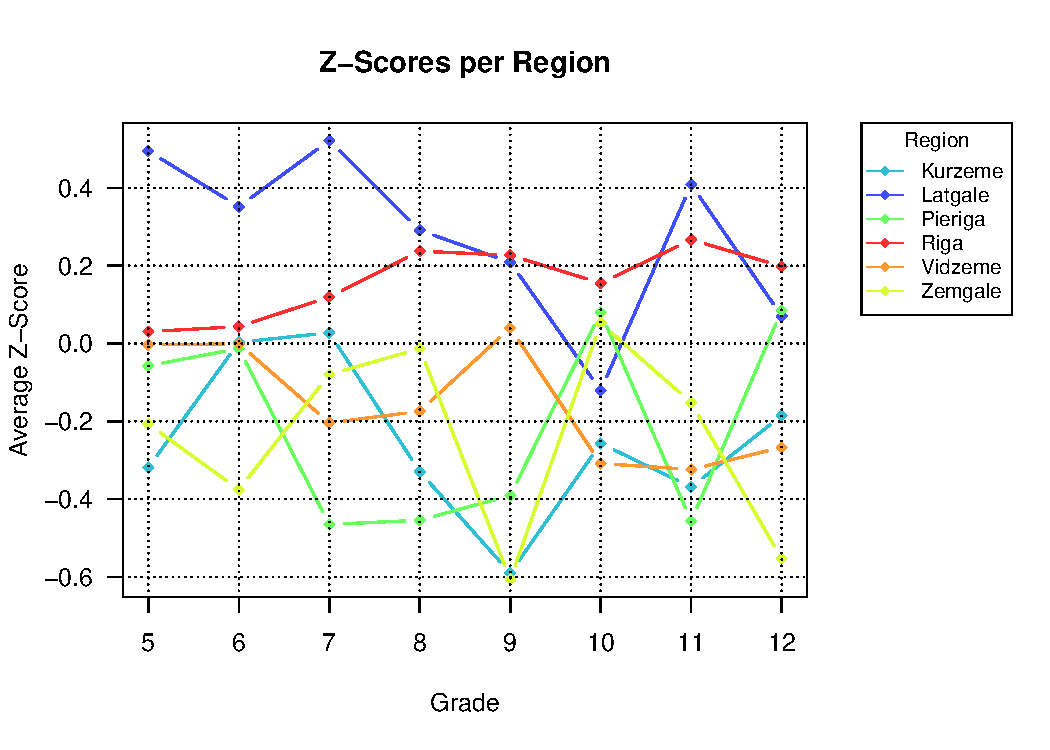
\includegraphics[width=\maxwidth]{figure/minimal-averages-per-region-1} 

}



\end{knitrout}



% 1+9+5 aktivitāšu skaitļi pa reģioniem
% Katram no 15 reģioniem dota dzimumu proporcija
%% Stabiņi grupās pa 3 - visi/meitenes/zēni. 

% 1+9+5 aktivitāšu skaitļi pa reģioniem - darbi latviešu valodā
% Katram no 15 reģioniem dota dzimumu proporcija

% 1+9+5 aktivitāšu skaitļi pa reģioniem - darbi krievu valodā
% Katram no 15 reģioniem dota dzimumu proporcija

\begin{knitrout}
\definecolor{shadecolor}{rgb}{0.969, 0.969, 0.969}\color{fgcolor}

{\centering 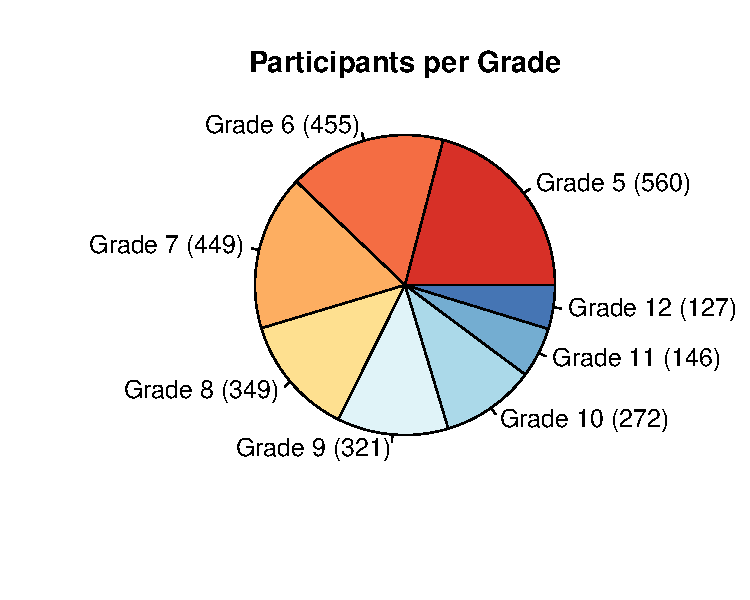
\includegraphics[width=\maxwidth]{figure/minimal-per-class-1} 

}



\end{knitrout}

\subsection{Dalība un sociāli-ekonomiskie rādītāji}

% Trīs 14-bumbulīšu diagrammas

Šeit varētu ievietot diagrammas pa novadiem vai novadu grupām, kas parāda divu parametru attiecību (varētu būt runa par burbulīšu diagrammām, ko zīmē divās dimensijās; turklāt burbulīša laukums ir aptuveni proporcionāls skolēnu skaitam olimpiādē).

\begin{itemize}
\item Sociāli-ekonomisko rādītāju --- bezdarbu, IIN uz 1 iedzīvotāju, pašvaldības izdevumus uz 1 skolēnu vai skolēnu skaitu skolā.
\item Dalībnieku aktivitāti (dalībnieku attiecību pret visiem skolēniem novadā) kā arī olimpiādes summāro rezultātu (punktu summas attiecību pret visiem skolēniem novadā). 
\end{itemize}

Šādas diagrammas palīdzētu saprast, kādi sociālie priekšnoteikumi veicina interesi par olimpiādēm, kāda izglītības politika (piemēram, mazo skolu saglabāšana vai slēgšana; lielāki vai mazāki izdevumi par vienu skolēnu) varētu pozitīvi iespaidot olimpiāžu rezultātus. 

\subsection{Dalībnieku struktūra}



%% Segmenti -- 6 NUTS reģioni
% http://en.wikipedia.org/wiki/Statistical_regions_of_Latvia

Atklātajā matemātikas olimpiādē sastopami darbi latviešu un krievu valodās. Valodu būtu visprecīzāk noteikt, aplūkojot katru konkrēto darbu. Par 41.\ AMO mums šādas informācijas nav, tādēļ valodu secinājām no skolēna re\v{g}istrācijā minētās informācijas, vai arī viņa skolā dominējošo valodu, bet jauktām skolām --- valodu, kas visbiežāk sastopama pieteiktā matemātikas skolotāja audzēkņu vidū. Katras klases joslas iekšpusē iezīmēts balts aplītis, kurš parāda latviešu skolēnu īpatsvaru visu attiecīgās klases audzēkņu vidū. Visām klašu grupām, izņemot 5.\ klasi, latviešu darbu īpatsvars 41.\ AMO ir nedaudz lielāks nekā skolēnu īpatsvars latviešu plūsmas skolās kopumā. Krievu valodā rakstošie skolēni olimpiādē piedalās nedaudz retāk, toties viņu rezultāti mēdz būt labāki (sk. apakšnodaļu "Pirmie 100 skolotāji pēc dalībnieku skaita augšējā kvartilē"). 

Kā redzams, dalība AMO nav pilnīgi proporcionāla latviešu un krievu skolu audzēkņu vidū. Tomēr atšķirības nav lielas --- pie pašreizējās olimpiādes apmeklētības, šo statistiku varētu jūtami izmainīt, papildus piesaistot dalībai olimpiādē dažus desmitus skolēnu. Latvijas vispārizglītojošajās skolās mācības mēdz notikt arī poļu, ukraiņu, baltkrievu, angļu un franču valodās. Šo skolu audzēkņi var izvēlēties rakstīt darbu latviski vai krieviski. Viņu darbi pieskaitīti atkarībā no re\v{g}istrācijā norādītās valodas.


%% K/L skaita attiecība pa klasēm 
\begin{knitrout}
\definecolor{shadecolor}{rgb}{0.969, 0.969, 0.969}\color{fgcolor}

{\centering 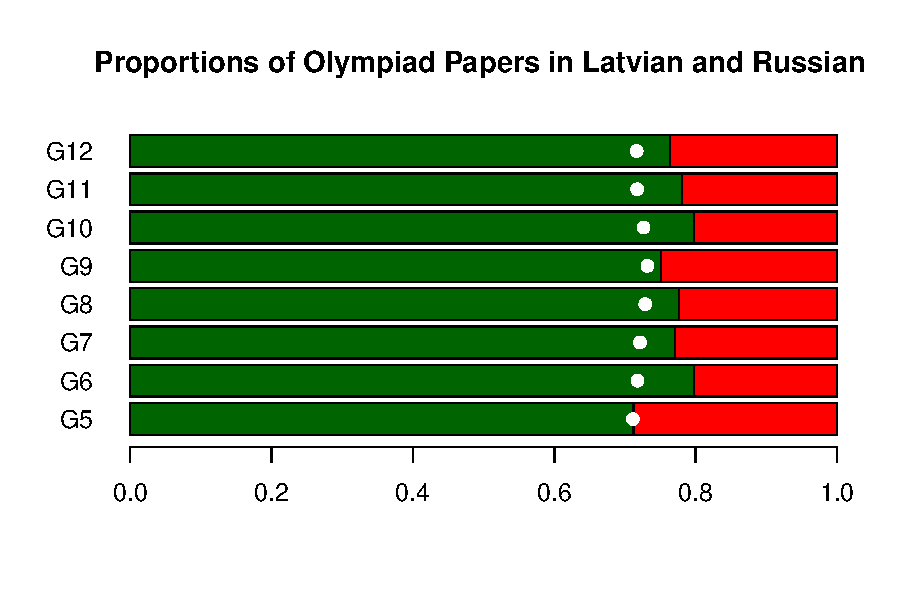
\includegraphics[width=\maxwidth]{figure/minimal-lang-proportions-1} 

}



\end{knitrout}



%% Marimekko diagrammas - dalībnieku dzimumu struktūra pa reģioniem. 
% https://learnr.wordpress.com/2009/03/29/ggplot2_marimekko_mosaic_chart/
%% Segmenti -- 4 urbanizācijas tipi (LV-meitenes, LV-zēni, RU-meitenes, RU-zēni)

Dalībnieku demogrāfisko struktūru var attēlot arī dažādām parametru kombinācijām. Šajā zīmējumā redzams dalībnieku sadalījums pa klasēm (vertikālie stabiņi), un katras klases iekšienē --- arī pa darbu valodām un dalībnieku dzimumiem. Skolēna dzimums re\v{g}istrācijas un rezultātu datos nav dots, 41.\ AMO tos noteicām pēc skolēna vārda. Pasaulē ir matemātikas sacensības, piemēram, EGMO (European Girls' Mathematical Olympiad), kuru nolūks ir veicināt meiteņu pievēršanos eksaktajām un inženierzinātnēm. Kopš olimpiādes pirmsākumiem (2012.\ gadā Kembridžā) EGMO piedalās arī četras vecāko klašu skolnieces no Latvijas. Sk. \url{https://www.egmo.org/}.

Latviešu valodā rakstītajiem darbiem zēnu un meiteņu ir aptuveni vienāds skaits, bet krievu valodā rakstītajiem darbiem meiteņu vecāko klašu grupās ir pat divreiz mazāk nekā zēnu.


\begin{knitrout}
\definecolor{shadecolor}{rgb}{0.969, 0.969, 0.969}\color{fgcolor}

{\centering 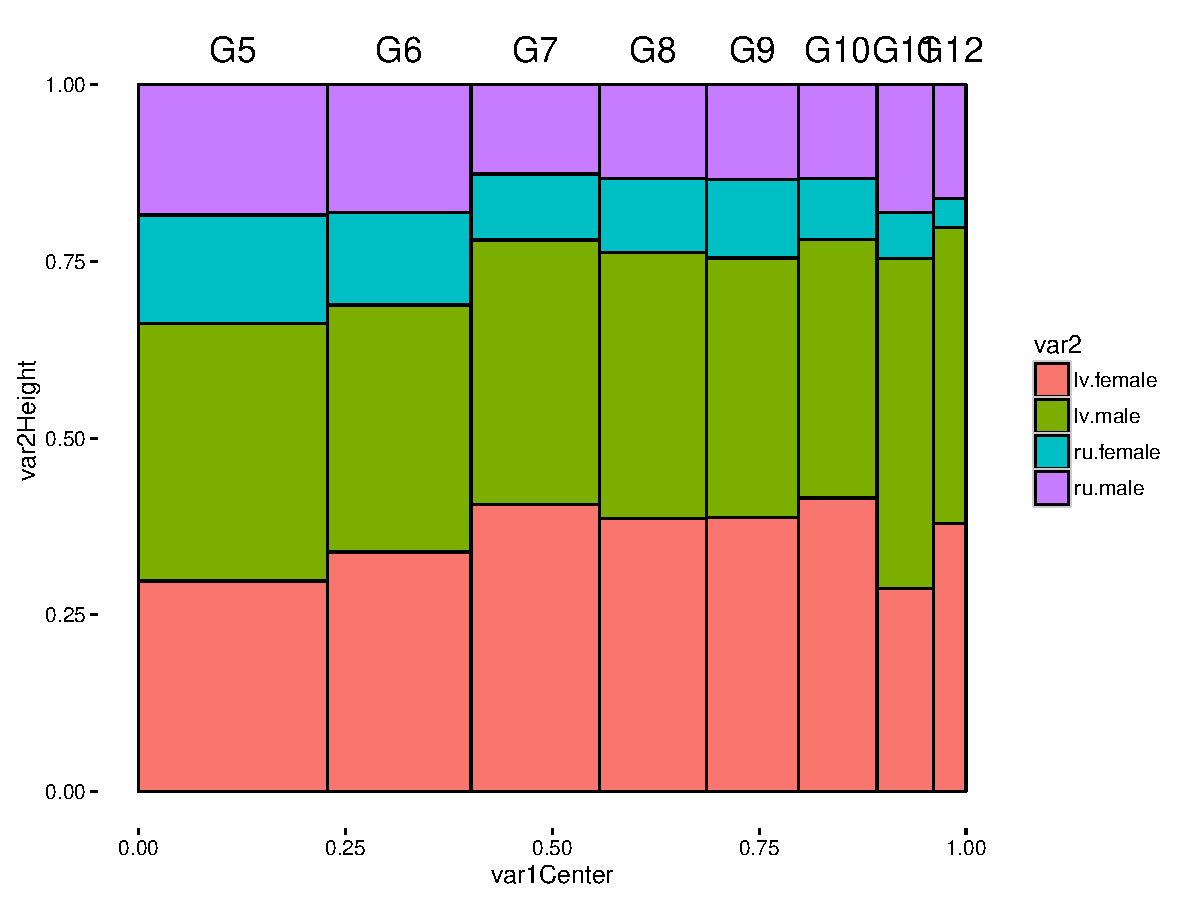
\includegraphics[width=\maxwidth]{figure/minimal-demography-segments-1} 

}



\end{knitrout}

\subsection{Dalībnieku valodas lielajās pilsētās}

Šajā diagrammā mazie aplīši parāda olimpiādes darbu valodu proporciju Latvijas lielākajās pilsētās (9 lielās pilsētas kā arī Ogre, Tukums un Cēsis, kurās iedzīvotāju skaits ir tuvu 20 tūkstošiem - t.i. daudz neatšķiras no Valmieras un Jēkabpils iedzīvotāju skaita). Aplīša laukums ir aptuveni proporcionāls dalībnieku skaitam no attiecīgās pilsētas.

\begin{knitrout}
\definecolor{shadecolor}{rgb}{0.969, 0.969, 0.969}\color{fgcolor}

{\centering 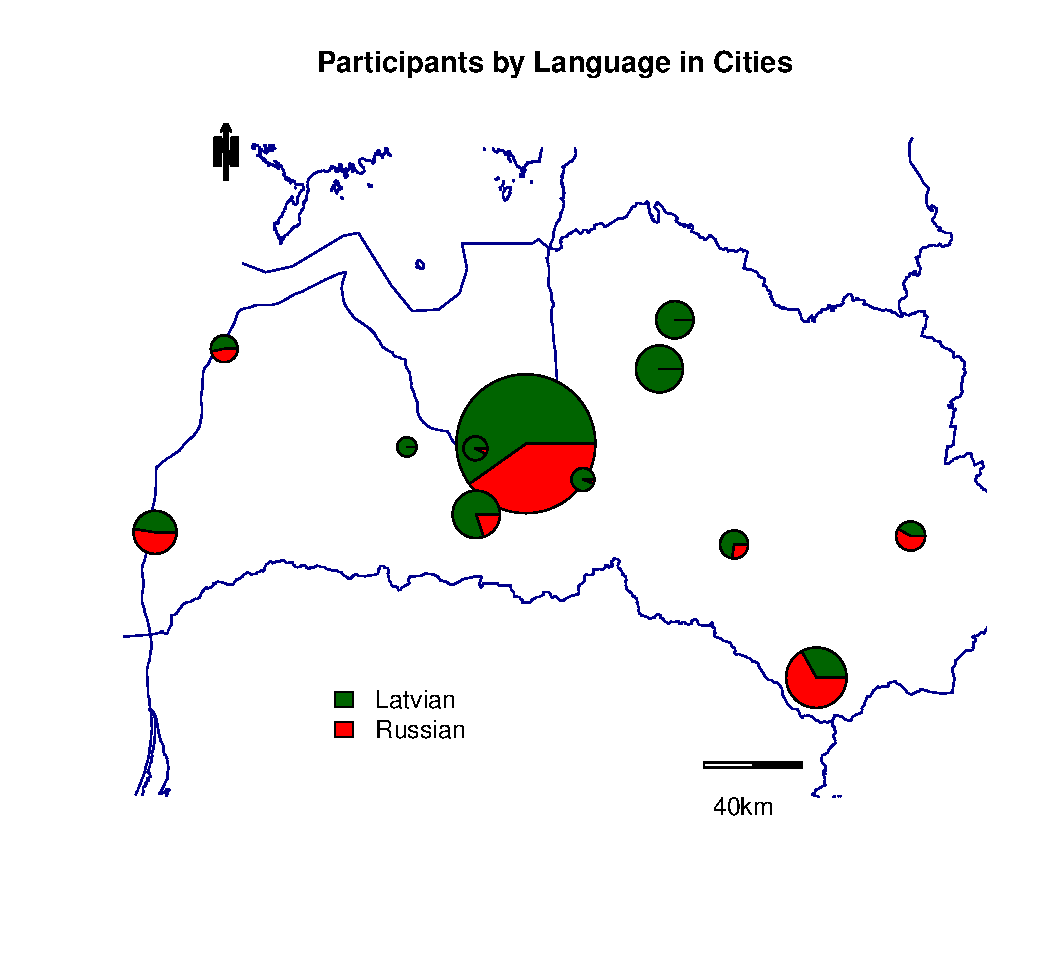
\includegraphics[width=\maxwidth]{figure/minimal-language-per-city-1} 

}



\end{knitrout}





\section{Vidējie rezultāti dalībnieku kategorijām}

Zīmējumā dots rezultātu intervāls katrai klasei. ``Kastītes'' kreisā mala atbilst apakšējai kvartilei, labā mala --- augšējai kvartilei, bet platā zilā svītriņa vidū --- mediānai. Ja klases darbus sakārtotu punktu pieaugšanas secībā un sadalītu četrās vienādās daļās, tad viszemāko punktu ieguvēju ceturtdaļa atrastos uz kreisās ūsas, divas vidējās ceturtdaļas --- kastītes iekšpusē, bet augšējā ceturtdaļa --- uz labās ūsas. Kā redzams attēlā, 12.\ klases skolnieku iegūtais punktu skaits ir būtiski lielāks nekā citu klašu risinātājiem. To varētu izskaidrot daži viegli uzdevumi, kuri ir 12.\ klases komplektā. 

\begin{knitrout}
\definecolor{shadecolor}{rgb}{0.969, 0.969, 0.969}\color{fgcolor}

{\centering 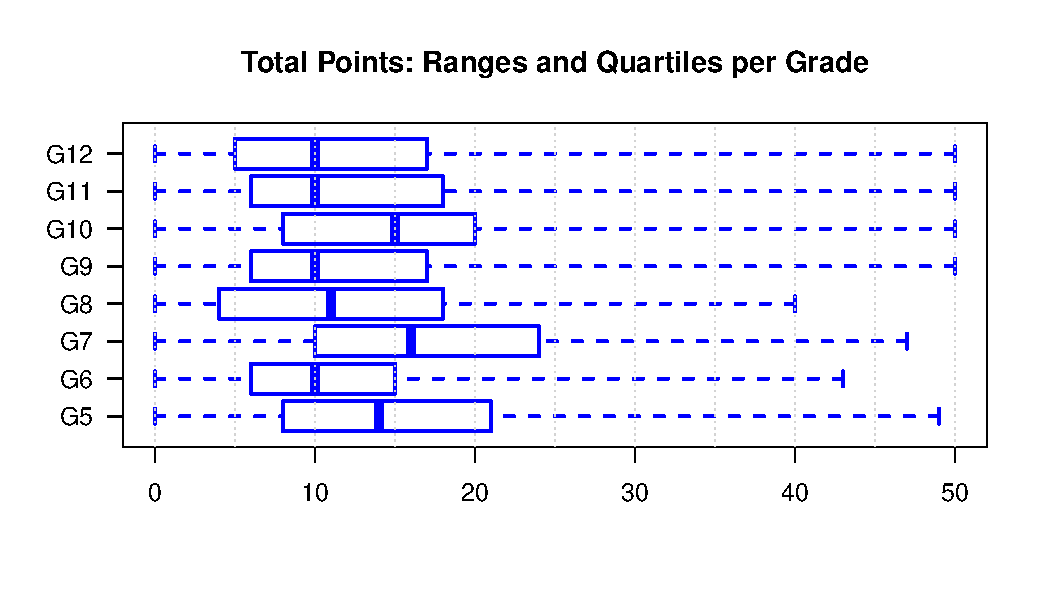
\includegraphics[width=\maxwidth]{figure/minimal-boxplots-per-grade-1} 

}



\end{knitrout}




%% Visu dalībnieku darbi, iekrāsotas godalgotās vietas 
%% Meiteņu un zēnu darbi (Meitenes zīmējam tanī pašā histogrammā)
%% Meitenes ir sazīmētas apakšā. 

%% Urbaniz. tips. Rīgas, 8 lielo pilsētu, mazpilsētu un lauku darbi

%% Latviešu un krievu valodā rakstītie darbi

%% Latviešu un krievu valodā rakstītie darbi -- tikai 9 lielajās pilsētās


\section{Skolas un skolotāji}



Tabulā apkopoti dati par matemātikas skolotājiem:

\noindent
{\bf Participants} --- Cik dalībnieku piedalījās olimpiādē.\\
{\bf Q3} --- Cik no viņiem ir ieguvuši rezultātu savas klases augšējā kvartilē. Punktu skaits, kas nepieciešams iekļūšanai augšējā kvartilē, ir atkarīgs no klases ($Q_3(Grade5)=21\;$, $Q_3(Grade6)=20\;$, $Q_3(Grade7)=18\;$, $Q_3(Grade8)=21\;$, $Q_3(Grade9)=24\;$, $Q_3(Grade10)=18\;$, $Q_3(Grade11)=15\;$, $Q_3(Grade12)=29\;$.)\\
{\bf Points} --- Kāda ir attiecīgā skolotāja sagatavoto skolēnu punktu summa.\\
{\bf School} --- Skolotāja pārstāvētā skola.



Tajos gadījumos, kad skolēns norādījis vairākus skolotājus, attiecīgo dalībnieku un viņa punktus pieskaita visiem skolotājiem. Kā redzams tabuliņā, vairums risinātāju (90.9\%) norādījuši tieši vienu skolotāju. 


\begin{knitrout}
\definecolor{shadecolor}{rgb}{0.969, 0.969, 0.969}\color{fgcolor}
\begin{tabular}{l|r}
\hline
Noraditi skolotaji & Darbu skaits\\
\hline
0 & 39\\
\hline
1 & 2434\\
\hline
2 & 202\\
\hline
3 & 4\\
\hline
Kopa & 2679\\
\hline
\end{tabular}


\end{knitrout}





Turpmākajās tabulās doti trīs dažādu veidu reitingi --- pirmie 100 skolotāji (pavisam bija 613 skolotāju, kuru vārdus skolēni norādīja savos darbos). Pirmajā reitingā skolotāji sakārtoti atbilstoši kopīgajam dalībnieku skaitam; otrajā reitingā --- atbilstoši dalībnieku skaitam, kuru rezultāts ir augšējā kvartilē, trešajā reitingā --- atbilstoši visu dalībnieku kopīgajam punktu skaitam. Šajos reitingos var ievērot, ka masveidīgākā dalība olimpiādēs ir skolēniem no Rīgas 1.\ \v{g}imnāzijas, savukārt pēc potenciālo laureātu un punktu skaita priekšgalā izvirzās Daugavpils Krievu vidusskola-licejs.

{\em Apzināti neveidojām reitingu pēc ``aritmētiskā vidējā rezultāta'', jo arī neliela punktu skaita saņemšana olimpiādē ir pozitīvs sasniegums; nebūtu attaisnojami tādi reitingi, kuros masveidīgāka dalība vilktu skolas vai skolotāja kopvērtējumu lejup.}


% Skolas pēc dalībnieku skaita

% Skolas pēc savāktajiem punktiem

%% Skolotāji pēc dalībnieku skaita

\newpage
{\bf Pirmie 100 skolotāji pēc dalībnieku skaita}\\ \nopagebreak
\begin{knitrout}
\definecolor{shadecolor}{rgb}{0.969, 0.969, 0.969}\color{fgcolor}
\begin{tabular}{r|l|r|r|r|l}
\hline
Num & Name & Participants & Q3 & Points & School\\
\hline
1 & Inese Lagzda & 54 & 22 & 873 & Rigas Valsts 1.gimnazija\\
\hline
2 & Daiga Jekabsone & 36 & 5 & 610 & Siguldas Valsts gimnazija\\
\hline
3 & Irena Oksenuka & 31 & 24 & 841 & Daugavpils Krievu vidusskola - licejs\\
\hline
4 & Karmena Liepina & 31 & 9 & 413 & Rigas Valsts 1.gimnazija\\
\hline
5 & Dzintars Zicans & 29 & 12 & 595 & Rigas Valsts 1.gimnazija\\
\hline
6 & Anita Indare & 26 & 6 & 292 & Jelgavas Spidolas gimnazija\\
\hline
7 & Dace Andzane & 24 & 13 & 607 & Rigas Valsts 1.gimnazija\\
\hline
8 & Vera Solovjova & 24 & 7 & 414 & Rigas 10.vidusskola\\
\hline
9 & Aija Vasilevska & 24 & 6 & 367 & Rigas Valsts 1.gimnazija\\
\hline
10 & Regina Simanovska & 23 & 13 & 565 & Rigas Valsts 1.gimnazija\\
\hline
11 & Zane Kaibe & 23 & 7 & 416 & Rigas 64.vidusskola\\
\hline
12 & Alesja Sapkova & 21 & 13 & 448 & Daugavpils Saskanas pamatskola\\
\hline
13 & Inese Lude & 21 & 5 & 285 & A.Pumpura Rigas 11.pamatskola\\
\hline
14 & Gunta Lace & 21 & 4 & 328 & Valmieras Valsts gimnazija\\
\hline
15 & Inese Boze & 20 & 5 & 240 & DA Cesu Valsts gimnazija\\
\hline
16 & Anita Slaidina & 19 & 12 & 436 & Cesu Valsts gimnazija\\
\hline
17 & Margita Jirgensone & 19 & 0 & 95 & Jelgavas Spidolas gimnazija\\
\hline
18 & Vita Brakovska & 18 & 9 & 446 & Rigas Valsts 1.gimnazija\\
\hline
19 & Ingrida Veilande & 17 & 5 & 294 & Adazu vidusskola\\
\hline
20 & Kristine Bezsapocnikova & 17 & 5 & 253 & Rigas 64.vidusskola\\
\hline
21 & Inga Neilande & 17 & 1 & 171 & Jelgavas 4.sakumskola\\
\hline
22 & Natalja Mosolova & 16 & 5 & 232 & Rigas 13.vidusskola\\
\hline
23 & Ligita Neimane & 16 & 4 & 235 & Cesu pilsetas pamatskola\\
\hline
24 & Agrita Bartusevica & 15 & 5 & 267 & Cesu Valsts gimnazija\\
\hline
25 & Dace Kuma & 15 & 4 & 261 & Dobeles Valsts gimnazija\\
\hline
26 & Anita Vabule & 15 & 3 & 242 & Madonas Valsts gimnazija\\
\hline
27 & Laila Ruke & 15 & 2 & 261 & Cesu Valsts gimnazija\\
\hline
28 & Rita Caunite & 15 & 1 & 243 & Rigas Francu licejs\\
\hline
29 & Viola Levina & 15 & 0 & 143 & Valkas gimnazija\\
\hline
30 & Ieva Ruksane & 15 & 0 & 74 & Limbazu novada gimnazija\\
\hline
31 & Maija Balode & 14 & 7 & 317 & Rigas Valsts 1.gimnazija\\
\hline
32 & Inta Ozolina & 14 & 4 & 230 & Siguldas pilsetas vidusskola\\
\hline
33 & Ineta Ivanova & 14 & 3 & 218 & Preilu Valsts gimnazija\\
\hline
34 & Sandra Kalnina & 14 & 1 & 134 & Ogres sakumskola\\
\hline
35 & Alina Magomedova & 13 & 11 & 347 & Daugavpils Krievu vidusskola - licejs\\
\hline
36 & Vaira Buza & 13 & 3 & 137 & DA Cesu Valsts gimnazija\\
\hline
37 & Liene Andzane & 13 & 2 & 148 & Kraslavas Valsts gimnazija\\
\hline
38 & Valentina Cesnokova & 13 & 1 & 170 & Rigas 13.vidusskola\\
\hline
39 & Inga Ruskule & 13 & 0 & 65 & Priekulu vidusskola\\
\hline
40 & Stanislav Didych & 12 & 9 & 256 & Daugavpils Krievu vidusskola - licejs\\
\hline
41 & Kristine Sevcenko & 12 & 6 & 230 & Rigas Valsts 1.gimnazija\\
\hline
42 & Aiva Rituma & 12 & 4 & 225 & Dobeles Valsts gimnazija\\
\hline
43 & Sandra Rubule & 12 & 3 & 164 & Jelgavas Valsts gimnazija\\
\hline
44 & Irina Iriscenko & 12 & 2 & 124 & Rigas 72.vidusskola\\
\hline
45 & Edite Teterovska & 12 & 1 & 174 & Rigas Lietuviesu vidusskola\\
\hline
46 & Ira Nikiforova & 12 & 1 & 158 & Plavinu novada gimnazija\\
\hline
47 & Ludmila Ulinska & 11 & 7 & 246 & Daugavpils Saskanas pamatskola\\
\hline
48 & Olga Sheremet & 11 & 5 & 196 & Rigas Zolitudes gimnazija\\
\hline
49 & Jelena Blagodarnaja & 11 & 3 & 204 & Rigas Purvciema vidusskola\\
\hline
50 & Andrejs Cibulis & 11 & 3 & 190 & Bauskas sakumskola\\
\hline
\end{tabular}


\end{knitrout}


\begin{knitrout}
\definecolor{shadecolor}{rgb}{0.969, 0.969, 0.969}\color{fgcolor}
\begin{tabular}{r|l|r|r|r|l}
\hline
Num & Name & Participants & Q3 & Points & School\\
\hline
51 & Nadezda Rjabinina & 11 & 3 & 142 & Rigas Zolitudes gimnazija\\
\hline
52 & Daina Denjuscenkova & 11 & 2 & 177 & Jelgavas 4.sakumskola\\
\hline
53 & Zaneta Kovalevska & 11 & 2 & 152 & Carnikavas pamatskola\\
\hline
54 & Lidija Lisovska & 11 & 1 & 144 & Cesu pilsetas pamatskola\\
\hline
55 & Dzintra Zingule & 11 & 0 & 85 & Jelgavas 3.sakumskola\\
\hline
56 & Irina Polakova & 10 & 7 & 290 & Daugavpils Krievu vidusskola - licejs\\
\hline
57 & Elina Fridmane & 10 & 5 & 234 & Rigas 64.vidusskola\\
\hline
58 & Nadezda Koleda & 10 & 5 & 224 & Rigas 34.vidusskola\\
\hline
59 & Irina Tarasova & 10 & 5 & 187 & Rigas 65.vidusskola\\
\hline
60 & Ruta Dubra & 10 & 2 & 130 & Ventspils 1.gimnazija\\
\hline
61 & Ilona Ivanova & 10 & 1 & 101 & Olaines 1.vidusskola\\
\hline
62 & Tatjana Strigalova & 10 & 0 & 100 & Rigas Valsts 2.gimnazija\\
\hline
63 & Gunta Kuzmina & 10 & 0 & 60 & Priekules vidusskola\\
\hline
64 & Rita Hrapane & 9 & 8 & 272 & Daugavpils Krievu vidusskola - licejs\\
\hline
65 & Jekaterina Klanovska & 9 & 5 & 230 & Daugavpils Krievu vidusskola - licejs\\
\hline
66 & Ilze Ose & 9 & 4 & 182 & Majoru vidusskola\\
\hline
67 & Inta Ungure & 9 & 4 & 175 & Rigas 25.vidusskola\\
\hline
68 & Veneranda Springe & 9 & 4 & 163 & Rudzatu vidusskola\\
\hline
69 & Sanita Birzniece & 9 & 4 & 160 & Tukuma 2.vidusskola\\
\hline
70 & Ligita Pickaine & 9 & 3 & 161 & Valmieras Valsts gimnazija\\
\hline
71 & Lilija Roldugina & 9 & 3 & 131 & Rigas 40.vidusskola\\
\hline
72 & Sandra Simanovica & 9 & 1 & 135 & Rigas 64.vidusskola\\
\hline
73 & Eva Lasmane & 9 & 0 & 135 & Valmieras sakumskola\\
\hline
74 & Agnese Suste & 9 & 0 & 84 & Materu Jura Kazdangas pamatskola\\
\hline
75 & Jolanta Saknere & 9 & 0 & 84 & Dobeles Valsts gimnazija\\
\hline
76 & Iveta Zarane & 8 & 6 & 162 & Daugavpils Krievu vidusskola - licejs\\
\hline
77 & Lilija Stunza & 8 & 5 & 201 & Rigas Zolitudes gimnazija\\
\hline
78 & Lidija Gaidamanova & 8 & 3 & 158 & Rigas Zolitudes gimnazija\\
\hline
79 & Valda Bickova & 8 & 3 & 158 & Uzvaras vidusskola\\
\hline
80 & Valentina Pavule & 8 & 2 & 148 & Rigas 40.vidusskola\\
\hline
81 & Jelena Kovalcuka & 8 & 2 & 129 & Rigas 88.vidusskola\\
\hline
82 & Sarma Rone & 8 & 2 & 95 & Jelgavas 4.sakumskola\\
\hline
83 & Tatjana Scogoleva & 8 & 1 & 126 & Puskina licejs\\
\hline
84 & Svetlana Proscinko & 8 & 1 & 118 & Daugavpils Valsts gimnazija\\
\hline
85 & Dzintra Bormane & 8 & 1 & 112 & Grundzales pamatskola\\
\hline
86 & Tatjana Kulikova & 8 & 1 & 94 & Rigas Herdera vidusskola\\
\hline
87 & Daiga Kravale & 8 & 0 & 71 & Jelgavas 4.sakumskola\\
\hline
88 & Inguna Kondratjeva & 8 & 0 & 70 & Smiltenes gimnazija\\
\hline
89 & Ligita Briede & 8 & 0 & 65 & Keguma komercnovirziena vidusskola\\
\hline
90 & Anita Jansone & 8 & 0 & 42 & Limbazu 3.vidusskola\\
\hline
91 & Annija Brezinska & 8 & 0 & 42 & Malpils novada vidusskola\\
\hline
92 & Vineta Troksa & 8 & 0 & 42 & Ventspils 6.vidusskola\\
\hline
93 & Vija Rasmane & 7 & 4 & 127 & A.Pumpura Rigas 11.pamatskola\\
\hline
94 & Valentina Paradovica & 7 & 3 & 132 & Rigas Klasiska gimnazija\\
\hline
95 & Tatjana Matrosova & 7 & 3 & 124 & Rigas 13.vidusskola\\
\hline
96 & Una Moiseja & 7 & 3 & 122 & Jaunmarupes sakumskola\\
\hline
97 & Kati Smotrova & 7 & 2 & 153 & Carnikavas pamatskola\\
\hline
98 & Laila Zinberga & 7 & 2 & 131 & Laurencu sakumskola\\
\hline
99 & Agnija Ruzule-Jaudzeme & 7 & 2 & 129 & Jurmalas Alternativa skola\\
\hline
100 & Elita Ritere & 7 & 2 & 127 & Rigas Valda Zalisa sakumskola\\
\hline
\end{tabular}


\end{knitrout}



\newpage
{\bf Pirmie 100 skolotāji pēc dalībnieku skaita augšējā kvartilē}\\ \nopagebreak
\begin{knitrout}
\definecolor{shadecolor}{rgb}{0.969, 0.969, 0.969}\color{fgcolor}
\begin{tabular}{r|l|r|r|r|l}
\hline
Num & Name & Participants & Q3 & Points & School\\
\hline
1 & Irena Oksenuka & 31 & 24 & 841 & Daugavpils Krievu vidusskola - licejs\\
\hline
2 & Inese Lagzda & 54 & 22 & 873 & Rigas Valsts 1.gimnazija\\
\hline
3 & Dace Andzane & 24 & 13 & 607 & Rigas Valsts 1.gimnazija\\
\hline
4 & Regina Simanovska & 23 & 13 & 565 & Rigas Valsts 1.gimnazija\\
\hline
5 & Alesja Sapkova & 21 & 13 & 448 & Daugavpils Saskanas pamatskola\\
\hline
6 & Dzintars Zicans & 29 & 12 & 595 & Rigas Valsts 1.gimnazija\\
\hline
7 & Anita Slaidina & 19 & 12 & 436 & Cesu Valsts gimnazija\\
\hline
8 & Alina Magomedova & 13 & 11 & 347 & Daugavpils Krievu vidusskola - licejs\\
\hline
9 & Karmena Liepina & 31 & 9 & 413 & Rigas Valsts 1.gimnazija\\
\hline
10 & Vita Brakovska & 18 & 9 & 446 & Rigas Valsts 1.gimnazija\\
\hline
11 & Stanislav Didych & 12 & 9 & 256 & Daugavpils Krievu vidusskola - licejs\\
\hline
12 & Rita Hrapane & 9 & 8 & 272 & Daugavpils Krievu vidusskola - licejs\\
\hline
13 & Vera Solovjova & 24 & 7 & 414 & Rigas 10.vidusskola\\
\hline
14 & Zane Kaibe & 23 & 7 & 416 & Rigas 64.vidusskola\\
\hline
15 & Maija Balode & 14 & 7 & 317 & Rigas Valsts 1.gimnazija\\
\hline
16 & Ludmila Ulinska & 11 & 7 & 246 & Daugavpils Saskanas pamatskola\\
\hline
17 & Irina Polakova & 10 & 7 & 290 & Daugavpils Krievu vidusskola - licejs\\
\hline
18 & Anita Indare & 26 & 6 & 292 & Jelgavas Spidolas gimnazija\\
\hline
19 & Aija Vasilevska & 24 & 6 & 367 & Rigas Valsts 1.gimnazija\\
\hline
20 & Kristine Sevcenko & 12 & 6 & 230 & Rigas Valsts 1.gimnazija\\
\hline
21 & Iveta Zarane & 8 & 6 & 162 & Daugavpils Krievu vidusskola - licejs\\
\hline
22 & Daiga Jekabsone & 36 & 5 & 610 & Siguldas Valsts gimnazija\\
\hline
23 & Inese Lude & 21 & 5 & 285 & A.Pumpura Rigas 11.pamatskola\\
\hline
24 & Inese Boze & 20 & 5 & 240 & DA Cesu Valsts gimnazija\\
\hline
25 & Ingrida Veilande & 17 & 5 & 294 & Adazu vidusskola\\
\hline
26 & Kristine Bezsapocnikova & 17 & 5 & 253 & Rigas 64.vidusskola\\
\hline
27 & Natalja Mosolova & 16 & 5 & 232 & Rigas 13.vidusskola\\
\hline
28 & Agrita Bartusevica & 15 & 5 & 267 & Cesu Valsts gimnazija\\
\hline
29 & Olga Sheremet & 11 & 5 & 196 & Rigas Zolitudes gimnazija\\
\hline
30 & Elina Fridmane & 10 & 5 & 234 & Rigas 64.vidusskola\\
\hline
31 & Nadezda Koleda & 10 & 5 & 224 & Rigas 34.vidusskola\\
\hline
32 & Irina Tarasova & 10 & 5 & 187 & Rigas 65.vidusskola\\
\hline
33 & Jekaterina Klanovska & 9 & 5 & 230 & Daugavpils Krievu vidusskola - licejs\\
\hline
34 & Lilija Stunza & 8 & 5 & 201 & Rigas Zolitudes gimnazija\\
\hline
35 & Anna Jansone & 5 & 5 & 144 & Rigas Valsts 1.gimnazija\\
\hline
36 & Gunta Lace & 21 & 4 & 328 & Valmieras Valsts gimnazija\\
\hline
37 & Ligita Neimane & 16 & 4 & 235 & Cesu pilsetas pamatskola\\
\hline
38 & Dace Kuma & 15 & 4 & 261 & Dobeles Valsts gimnazija\\
\hline
39 & Inta Ozolina & 14 & 4 & 230 & Siguldas pilsetas vidusskola\\
\hline
40 & Aiva Rituma & 12 & 4 & 225 & Dobeles Valsts gimnazija\\
\hline
41 & Ilze Ose & 9 & 4 & 182 & Majoru vidusskola\\
\hline
42 & Inta Ungure & 9 & 4 & 175 & Rigas 25.vidusskola\\
\hline
43 & Veneranda Springe & 9 & 4 & 163 & Rudzatu vidusskola\\
\hline
44 & Sanita Birzniece & 9 & 4 & 160 & Tukuma 2.vidusskola\\
\hline
45 & Vija Rasmane & 7 & 4 & 127 & A.Pumpura Rigas 11.pamatskola\\
\hline
46 & Boriss Koltuns & 5 & 4 & 144 & Daugavpils Krievu vidusskola - licejs\\
\hline
47 & Svetlana Elksnina & 5 & 4 & 138 & Daugavpils Krievu vidusskola - licejs\\
\hline
48 & Inna Kononova & 4 & 4 & 109 & Daugavpils Krievu vidusskola - licejs\\
\hline
49 & Vanda Lovcinovska & 4 & 4 & 98 & Jekabpils 2.vidusskola\\
\hline
50 & Anita Vabule & 15 & 3 & 242 & Madonas Valsts gimnazija\\
\hline
\end{tabular}


\end{knitrout}


\begin{knitrout}
\definecolor{shadecolor}{rgb}{0.969, 0.969, 0.969}\color{fgcolor}
\begin{tabular}{r|l|r|r|r|l}
\hline
Num & Name & Participants & Q3 & Points & School\\
\hline
51 & Ineta Ivanova & 14 & 3 & 218 & Preilu Valsts gimnazija\\
\hline
52 & Vaira Buza & 13 & 3 & 137 & DA Cesu Valsts gimnazija\\
\hline
53 & Sandra Rubule & 12 & 3 & 164 & Jelgavas Valsts gimnazija\\
\hline
54 & Jelena Blagodarnaja & 11 & 3 & 204 & Rigas Purvciema vidusskola\\
\hline
55 & Andrejs Cibulis & 11 & 3 & 190 & Bauskas sakumskola\\
\hline
56 & Nadezda Rjabinina & 11 & 3 & 142 & Rigas Zolitudes gimnazija\\
\hline
57 & Ligita Pickaine & 9 & 3 & 161 & Valmieras Valsts gimnazija\\
\hline
58 & Lilija Roldugina & 9 & 3 & 131 & Rigas 40.vidusskola\\
\hline
59 & Lidija Gaidamanova & 8 & 3 & 158 & Rigas Zolitudes gimnazija\\
\hline
60 & Valda Bickova & 8 & 3 & 158 & Uzvaras vidusskola\\
\hline
61 & Valentina Paradovica & 7 & 3 & 132 & Rigas Klasiska gimnazija\\
\hline
62 & Tatjana Matrosova & 7 & 3 & 124 & Rigas 13.vidusskola\\
\hline
63 & Una Moiseja & 7 & 3 & 122 & Jaunmarupes sakumskola\\
\hline
64 & Maira Tuklere & 6 & 3 & 133 & Rigas Natalijas Draudzinas vidusskola\\
\hline
65 & Inga Upeniece & 6 & 3 & 125 & Agenskalna Valsts gimnazija\\
\hline
66 & Sanita Eglite & 6 & 3 & 106 & Valmieras sakumskola\\
\hline
67 & Alla Kitajeva & 6 & 3 & 105 & Ventspils 2.vidusskola\\
\hline
68 & Romualda Gavsina & 6 & 3 & 94 & Rigas 88.vidusskola\\
\hline
69 & Irena Kozlovska & 6 & 3 & 88 & Puskina licejs\\
\hline
70 & Aleksandra Gulane & 5 & 3 & 139 & Rigas 40.vidusskola\\
\hline
71 & Galina Kozane & 5 & 3 & 91 & Rigas 22.vidusskola\\
\hline
72 & Elita Vaivode & 4 & 3 & 130 & Livanu 1.vidusskola\\
\hline
73 & Laila Aigare & 4 & 3 & 120 & Rigas Valda Zalisa sakumskola\\
\hline
74 & Linda Krastina & 4 & 3 & 103 & Salaspils 1.vidusskola\\
\hline
75 & Valentina Kapteine & 4 & 3 & 76 & Rigas 10.vidusskola\\
\hline
76 & Vita Brauna & 3 & 3 & 91 & Ogres 1.vidusskola\\
\hline
77 & Sigita Rathena & 3 & 3 & 90 & Talsu Kristiga vidusskola\\
\hline
78 & Laila Ruke & 15 & 2 & 261 & Cesu Valsts gimnazija\\
\hline
79 & Liene Andzane & 13 & 2 & 148 & Kraslavas Valsts gimnazija\\
\hline
80 & Irina Iriscenko & 12 & 2 & 124 & Rigas 72.vidusskola\\
\hline
81 & Daina Denjuscenkova & 11 & 2 & 177 & Jelgavas 4.sakumskola\\
\hline
82 & Zaneta Kovalevska & 11 & 2 & 152 & Carnikavas pamatskola\\
\hline
83 & Ruta Dubra & 10 & 2 & 130 & Ventspils 1.gimnazija\\
\hline
84 & Valentina Pavule & 8 & 2 & 148 & Rigas 40.vidusskola\\
\hline
85 & Jelena Kovalcuka & 8 & 2 & 129 & Rigas 88.vidusskola\\
\hline
86 & Sarma Rone & 8 & 2 & 95 & Jelgavas 4.sakumskola\\
\hline
87 & Kati Smotrova & 7 & 2 & 153 & Carnikavas pamatskola\\
\hline
88 & Laila Zinberga & 7 & 2 & 131 & Laurencu sakumskola\\
\hline
89 & Agnija Ruzule-Jaudzeme & 7 & 2 & 129 & Jurmalas Alternativa skola\\
\hline
90 & Elita Ritere & 7 & 2 & 127 & Rigas Valda Zalisa sakumskola\\
\hline
91 & Edite Jeruma & 7 & 2 & 123 & Rigas 45.vidusskola\\
\hline
92 & Anita Porina & 7 & 2 & 101 & Grobinas gimnazija\\
\hline
93 & Svetlana Saveiko & 7 & 2 & 86 & Rigas 40.vidusskola\\
\hline
94 & Irina Kravcenko & 6 & 2 & 141 & Puskina licejs\\
\hline
95 & Ilze Vitina & 6 & 2 & 126 & Sakumskola Taurenitis\\
\hline
96 & Indra Upite-Dambite & 6 & 2 & 125 & Siguldas Valsts gimnazija\\
\hline
97 & Anita Upeniece & 6 & 2 & 115 & Rigas 45.vidusskola\\
\hline
98 & Laila Kampe & 6 & 2 & 113 & E.Darzina muzikas vidusskola\\
\hline
99 & Sarma Jekabsone & 6 & 2 & 111 & Adazu vidusskola\\
\hline
100 & Natalja Jegorova & 6 & 2 & 110 & Rigas Klasiska gimnazija\\
\hline
\end{tabular}


\end{knitrout}



\newpage
{\bf Pirmie 100 skolotāji pēc visu dalībnieku punktu kopskaita}\\ \nopagebreak
\begin{knitrout}
\definecolor{shadecolor}{rgb}{0.969, 0.969, 0.969}\color{fgcolor}
\begin{tabular}{r|l|r|r|r|l}
\hline
Num & Name & Participants & Q3 & Points & School\\
\hline
1 & Inese Lagzda & 54 & 22 & 873 & Rigas Valsts 1.gimnazija\\
\hline
2 & Irena Oksenuka & 31 & 24 & 841 & Daugavpils Krievu vidusskola - licejs\\
\hline
3 & Daiga Jekabsone & 36 & 5 & 610 & Siguldas Valsts gimnazija\\
\hline
4 & Dace Andzane & 24 & 13 & 607 & Rigas Valsts 1.gimnazija\\
\hline
5 & Dzintars Zicans & 29 & 12 & 595 & Rigas Valsts 1.gimnazija\\
\hline
6 & Regina Simanovska & 23 & 13 & 565 & Rigas Valsts 1.gimnazija\\
\hline
7 & Alesja Sapkova & 21 & 13 & 448 & Daugavpils Saskanas pamatskola\\
\hline
8 & Vita Brakovska & 18 & 9 & 446 & Rigas Valsts 1.gimnazija\\
\hline
9 & Anita Slaidina & 19 & 12 & 436 & Cesu Valsts gimnazija\\
\hline
10 & Zane Kaibe & 23 & 7 & 416 & Rigas 64.vidusskola\\
\hline
11 & Vera Solovjova & 24 & 7 & 414 & Rigas 10.vidusskola\\
\hline
12 & Karmena Liepina & 31 & 9 & 413 & Rigas Valsts 1.gimnazija\\
\hline
13 & Aija Vasilevska & 24 & 6 & 367 & Rigas Valsts 1.gimnazija\\
\hline
14 & Alina Magomedova & 13 & 11 & 347 & Daugavpils Krievu vidusskola - licejs\\
\hline
15 & Gunta Lace & 21 & 4 & 328 & Valmieras Valsts gimnazija\\
\hline
16 & Maija Balode & 14 & 7 & 317 & Rigas Valsts 1.gimnazija\\
\hline
17 & Ingrida Veilande & 17 & 5 & 294 & Adazu vidusskola\\
\hline
18 & Anita Indare & 26 & 6 & 292 & Jelgavas Spidolas gimnazija\\
\hline
19 & Irina Polakova & 10 & 7 & 290 & Daugavpils Krievu vidusskola - licejs\\
\hline
20 & Inese Lude & 21 & 5 & 285 & A.Pumpura Rigas 11.pamatskola\\
\hline
21 & Rita Hrapane & 9 & 8 & 272 & Daugavpils Krievu vidusskola - licejs\\
\hline
22 & Agrita Bartusevica & 15 & 5 & 267 & Cesu Valsts gimnazija\\
\hline
23 & Dace Kuma & 15 & 4 & 261 & Dobeles Valsts gimnazija\\
\hline
24 & Laila Ruke & 15 & 2 & 261 & Cesu Valsts gimnazija\\
\hline
25 & Stanislav Didych & 12 & 9 & 256 & Daugavpils Krievu vidusskola - licejs\\
\hline
26 & Kristine Bezsapocnikova & 17 & 5 & 253 & Rigas 64.vidusskola\\
\hline
27 & Ludmila Ulinska & 11 & 7 & 246 & Daugavpils Saskanas pamatskola\\
\hline
28 & Rita Caunite & 15 & 1 & 243 & Rigas Francu licejs\\
\hline
29 & Anita Vabule & 15 & 3 & 242 & Madonas Valsts gimnazija\\
\hline
30 & Inese Boze & 20 & 5 & 240 & DA Cesu Valsts gimnazija\\
\hline
31 & Ligita Neimane & 16 & 4 & 235 & Cesu pilsetas pamatskola\\
\hline
32 & Elina Fridmane & 10 & 5 & 234 & Rigas 64.vidusskola\\
\hline
33 & Natalja Mosolova & 16 & 5 & 232 & Rigas 13.vidusskola\\
\hline
34 & Inta Ozolina & 14 & 4 & 230 & Siguldas pilsetas vidusskola\\
\hline
35 & Kristine Sevcenko & 12 & 6 & 230 & Rigas Valsts 1.gimnazija\\
\hline
36 & Jekaterina Klanovska & 9 & 5 & 230 & Daugavpils Krievu vidusskola - licejs\\
\hline
37 & Aiva Rituma & 12 & 4 & 225 & Dobeles Valsts gimnazija\\
\hline
38 & Nadezda Koleda & 10 & 5 & 224 & Rigas 34.vidusskola\\
\hline
39 & Ineta Ivanova & 14 & 3 & 218 & Preilu Valsts gimnazija\\
\hline
40 & Jelena Blagodarnaja & 11 & 3 & 204 & Rigas Purvciema vidusskola\\
\hline
41 & Lilija Stunza & 8 & 5 & 201 & Rigas Zolitudes gimnazija\\
\hline
42 & Olga Sheremet & 11 & 5 & 196 & Rigas Zolitudes gimnazija\\
\hline
43 & Andrejs Cibulis & 11 & 3 & 190 & Bauskas sakumskola\\
\hline
44 & Irina Tarasova & 10 & 5 & 187 & Rigas 65.vidusskola\\
\hline
45 & Ilze Ose & 9 & 4 & 182 & Majoru vidusskola\\
\hline
46 & Daina Denjuscenkova & 11 & 2 & 177 & Jelgavas 4.sakumskola\\
\hline
47 & Inta Ungure & 9 & 4 & 175 & Rigas 25.vidusskola\\
\hline
48 & Edite Teterovska & 12 & 1 & 174 & Rigas Lietuviesu vidusskola\\
\hline
49 & Inga Neilande & 17 & 1 & 171 & Jelgavas 4.sakumskola\\
\hline
50 & Valentina Cesnokova & 13 & 1 & 170 & Rigas 13.vidusskola\\
\hline
\end{tabular}


\end{knitrout}


\begin{knitrout}
\definecolor{shadecolor}{rgb}{0.969, 0.969, 0.969}\color{fgcolor}
\begin{tabular}{r|l|r|r|r|l}
\hline
Num & Name & Participants & Q3 & Points & School\\
\hline
51 & Sandra Rubule & 12 & 3 & 164 & Jelgavas Valsts gimnazija\\
\hline
52 & Veneranda Springe & 9 & 4 & 163 & Rudzatu vidusskola\\
\hline
53 & Iveta Zarane & 8 & 6 & 162 & Daugavpils Krievu vidusskola - licejs\\
\hline
54 & Ligita Pickaine & 9 & 3 & 161 & Valmieras Valsts gimnazija\\
\hline
55 & Sanita Birzniece & 9 & 4 & 160 & Tukuma 2.vidusskola\\
\hline
56 & Ira Nikiforova & 12 & 1 & 158 & Plavinu novada gimnazija\\
\hline
57 & Lidija Gaidamanova & 8 & 3 & 158 & Rigas Zolitudes gimnazija\\
\hline
58 & Valda Bickova & 8 & 3 & 158 & Uzvaras vidusskola\\
\hline
59 & Kati Smotrova & 7 & 2 & 153 & Carnikavas pamatskola\\
\hline
60 & Zaneta Kovalevska & 11 & 2 & 152 & Carnikavas pamatskola\\
\hline
61 & Liene Andzane & 13 & 2 & 148 & Kraslavas Valsts gimnazija\\
\hline
62 & Valentina Pavule & 8 & 2 & 148 & Rigas 40.vidusskola\\
\hline
63 & Lidija Lisovska & 11 & 1 & 144 & Cesu pilsetas pamatskola\\
\hline
64 & Anna Jansone & 5 & 5 & 144 & Rigas Valsts 1.gimnazija\\
\hline
65 & Boriss Koltuns & 5 & 4 & 144 & Daugavpils Krievu vidusskola - licejs\\
\hline
66 & Viola Levina & 15 & 0 & 143 & Valkas gimnazija\\
\hline
67 & Nadezda Rjabinina & 11 & 3 & 142 & Rigas Zolitudes gimnazija\\
\hline
68 & Irina Kravcenko & 6 & 2 & 141 & Puskina licejs\\
\hline
69 & Aleksandra Gulane & 5 & 3 & 139 & Rigas 40.vidusskola\\
\hline
70 & Svetlana Elksnina & 5 & 4 & 138 & Daugavpils Krievu vidusskola - licejs\\
\hline
71 & Vaira Buza & 13 & 3 & 137 & DA Cesu Valsts gimnazija\\
\hline
72 & Sandra Simanovica & 9 & 1 & 135 & Rigas 64.vidusskola\\
\hline
73 & Eva Lasmane & 9 & 0 & 135 & Valmieras sakumskola\\
\hline
74 & Sandra Kalnina & 14 & 1 & 134 & Ogres sakumskola\\
\hline
75 & Maira Tuklere & 6 & 3 & 133 & Rigas Natalijas Draudzinas vidusskola\\
\hline
76 & Valentina Paradovica & 7 & 3 & 132 & Rigas Klasiska gimnazija\\
\hline
77 & Lilija Roldugina & 9 & 3 & 131 & Rigas 40.vidusskola\\
\hline
78 & Laila Zinberga & 7 & 2 & 131 & Laurencu sakumskola\\
\hline
79 & Ruta Dubra & 10 & 2 & 130 & Ventspils 1.gimnazija\\
\hline
80 & Elita Vaivode & 4 & 3 & 130 & Livanu 1.vidusskola\\
\hline
81 & Jelena Kovalcuka & 8 & 2 & 129 & Rigas 88.vidusskola\\
\hline
82 & Agnija Ruzule-Jaudzeme & 7 & 2 & 129 & Jurmalas Alternativa skola\\
\hline
83 & Vija Rasmane & 7 & 4 & 127 & A.Pumpura Rigas 11.pamatskola\\
\hline
84 & Elita Ritere & 7 & 2 & 127 & Rigas Valda Zalisa sakumskola\\
\hline
85 & Tatjana Scogoleva & 8 & 1 & 126 & Puskina licejs\\
\hline
86 & Ilze Vitina & 6 & 2 & 126 & Sakumskola Taurenitis\\
\hline
87 & Inga Upeniece & 6 & 3 & 125 & Agenskalna Valsts gimnazija\\
\hline
88 & Indra Upite-Dambite & 6 & 2 & 125 & Siguldas Valsts gimnazija\\
\hline
89 & Inta Laicane & 5 & 2 & 125 & Ogres 1.vidusskola\\
\hline
90 & Irina Iriscenko & 12 & 2 & 124 & Rigas 72.vidusskola\\
\hline
91 & Tatjana Matrosova & 7 & 3 & 124 & Rigas 13.vidusskola\\
\hline
92 & Edite Jeruma & 7 & 2 & 123 & Rigas 45.vidusskola\\
\hline
93 & Una Moiseja & 7 & 3 & 122 & Jaunmarupes sakumskola\\
\hline
94 & Biruta Caune & 7 & 1 & 121 & Rigas 64.vidusskola\\
\hline
95 & Tatjana Petuhova & 7 & 1 & 120 & Rigas 95.vidusskola\\
\hline
96 & Laila Aigare & 4 & 3 & 120 & Rigas Valda Zalisa sakumskola\\
\hline
97 & Svetlana Proscinko & 8 & 1 & 118 & Daugavpils Valsts gimnazija\\
\hline
98 & Anita Upeniece & 6 & 2 & 115 & Rigas 45.vidusskola\\
\hline
99 & Jelena Grincisina & 5 & 2 & 114 & Daugavpils 3.vidusskola\\
\hline
100 & Nonna Anohina & 5 & 1 & 114 & Jelgavas 2.pamatskola\\
\hline
\end{tabular}


\end{knitrout}


\subsection{``Nevienlīdzība'' un Džini koeficienti}

Viegli redzēt, ka skolēnu izredzes olimpiādē būtiski atšķiras no izvēlētā matemātikas skolotāja, skolas un arī no pašvaldības. Šajā apakšnodaļā mē\v{g}ināsim saprast, cik lielā mērā varbūtība piedalīties olimpiādē, izredzes iegūt godalgotu vietu (mūsu aprēķinos --- atrašanās augšējā kvartilē) un arī iegūtais punktu skaits ir sadalīti nevienlīdzīgi starp skolotāju audzēkņiem. Ņemot vērā to, ka labākie olimpiāžu rezultāti ir sakoncentrēti nedaudzās skolās, šādu nevienlīdzību nevar pilnībā izskaidrot ar skolotāju prasmēm vien, bet gan ar bērnu atlasi.  

\noindent
{\bf Atskaites punkts: Skaitliska ``vienlīdzības'' simulācija.} Protams, pilnīga vienlīdzība nav nedz sasniedzama, nedz arī vēlama. Lai Džini koeficientu aprēķinam rastos kāds atskaites punkts, izdarīsim virkni pieņēmumu par to, kā izglītība ir organizēta hipotētiskā valstī Aizspogulijā, kur ir līdzīga skolēnu un skolotāju demogrāfija, bet olimpiādes rezultāts atspoguļo vienīgi skolēnu matemātiskās spējas. Ja mums rastos iespēja salīdzināt Latvijā pastāvošo rezultātu nevienlīdzību ar kādu reālu valsti, tad Aizspoguliju varētu aizstāt ar kādu reālu piemēru.

\begin{itemize}
\item Aizspogulijā dzīvo 120000 skolēnu, kas mācās no 5.\ līdz 12.\ klasei. 
\item Katra Aizspogulijas skolotāja vai pulciņa vadītāja pārraudzībā esošo skolēnu skaits ir nejaušs, vienmērīgi sadalīts vesels skaitlis no 0 līdz 100. (Pavisam Aizspogulijā ir 2400 matemātikas skolotāju --- vidēji pa vienam uz katriem 50 skolēniem.)
\item Aptuveni 2\% no Aizspogulijas skolēniem vēlas piedalīties matemātikas olimpiādē. 
\item Visā Aizspogulijā skolēniem ir līdzīgas iespējas sagatavoties olimpiādei, olimpiādes rezultāts atspoguļo nevis skolotāja, skolas vai pašvaldības izvēli, bet ir atkarīgs no skolēna dotumiem (matemātiska apdāvinātība, spēja pierakstīt risinājumus, mērķtiecīga gatavošanās, utml.) Olimpiādē saņemtie punkti ir sadalīti ar {\em nogriezto normālo sadalījumu} ({\em truncated normal distribution}) ar vidējo vērtību $\mu = 15$, standartnovirzi $\sigma = 10$ un vērtībām intervālā $[0,50]$.
\item Jebkuram skolēnam ir vienādas izredzes nokļūt pie jebkura skolotāja; nenotiek skolēnu stratifikācija atkarībā no mācību rezultātiem. 
\end{itemize}

Šajā piemērā Aizspogulijas skaitliskie lielumi (skolēnu un matemātikas skolotāju skaits; punktu sadalījums olimpiādē) aptuveni atbilst Latvijas situācijai, tomēr nepastāv skolēnu šķirošana. Aizspogulijas rādījumus Džini koeficientam ņemsim par atskaites punktu, lai varētu salīzināt, par kādu daļu Latvijā pastāvošās iespējas gatavoties olimpiādēm ir nevienlīdzīgākas. (Nebūtu jēgas salīdzināt ar Džini koeficientu 0, jo tas nozīmētu olimpiāžu dalībnieku un viņu punktu absolūti vienādu sadalījumu starp skolotājiem, kas ir mazticami pat ar Aizspogulijas pieņēmumiem.) 

To nevienlīdzību (pareizāk sakot - galaiznākumu nevienādību), kas rodas Aizspogulijā varbūtisko sadalījumu ieviesto nejaušību rezultātā iegūsim, izmantojot skaitlisku olimpiādes rezultātu simulāciju. Katram no 2400 skolotājiem piešķiram nejaušu skolēnu skaitu no 0 līdz 100; katrs skolēns piedalās Bernulli eksperimentā (ar varbūtību 2\% piedalās olimpiādē); visbeidzot katrs olimpiādes dalībnieks iegūst punktu kopskaitu atbilstoši nogrieztajam normālajam sadalījumam. Šādi iegūtajiem datiem aprēķinām tās pašas Lorenca līknes un Džini koeficientus.

\noindent
{\bf Lorenca līkne dalībnieku skaita, augšējās kvartiles dalībnieku skaita un punktu summas sadalījumam starp skolotājiem Latvijā:}

\begin{knitrout}
\definecolor{shadecolor}{rgb}{0.969, 0.969, 0.969}\color{fgcolor}

{\centering \includegraphics[width=\maxwidth]{figure/minimal-gini1-1} 

}



\end{knitrout}

\noindent
{\bf Lorenca līkne dalībnieku skaita, augšējās kvartiles dalībnieku skaita un punktu summas sadalījumam starp skolotājiem Aizspogulijā (olimpiādes rezultātu vietā skaitliska simulācija):}

\begin{knitrout}
\definecolor{shadecolor}{rgb}{0.969, 0.969, 0.969}\color{fgcolor}

{\centering \includegraphics[width=\maxwidth]{figure/minimal-gini2-1} 

}



\end{knitrout}


\begin{knitrout}
\definecolor{shadecolor}{rgb}{0.969, 0.969, 0.969}\color{fgcolor}
\begin{tabular}{l|r|r}
\hline
Measurement Type & Gini for Latvia & Gini for Looking-Glass Land\\
\hline
Participants & 0.478 & 0.278\\
\hline
Q3 & 0.721 & 0.656\\
\hline
Points & 0.541 & 0.371\\
\hline
\end{tabular}


\end{knitrout}

Kā redzams no Lorenca līknēm, nevienlīdzība matemātiskajās olimpiādēs izpaužas ļoti jūtamā veidā: 20\% skolotāju ar zemāko skaitu olimpiādei sagatavoto skolēnu nodrošina tikai 4\% no olimpiādes dalībnieku kopskaita (un šeit netiek ieskaitīti tie skolotāji, kuri skolēnus olimpiādei negatavo vispār; tostarp no tām 50 Latvijas pašvaldībām, kas 41.\ atklātajā matemātikas olimpiādē nebija pārstāvētas).

Arī Aizspogulijas simulācijā būtu ievērojama nevienlīdzība starp to, cik potenciālos olimpiāžu laureātus (risinātājus, kuru rezultāts ir augšējā kvartilē) sagatavotu katrs skolotājs; tomēr jāņem vērā, ka šajā simulācijā daudz lielāks skaits skolotāju nosūtītu uz olimpiādi vismaz vienu dalībnieku: Latvijā 41.\ matemātikas olimpiādē bija pārstāvēti 613 skolotāji, savukārt Aizspogulijā tādu būtu 1366. Ja skolotāju iesaiste olimpiādē ir līdzīgāka un vidējais audzēkņu skaits uz vienu skolotāju ir mazāks, tad ir pašsaprotami, ka liela daļa no viņiem nesagatavos nevienu laureātu. No šejienes izriet secinājums, ka skolu darbu nebūtu pareizi salīdzināt pēc sagatavoto olimpiāžu laureātu skaita --- it īpaši, ja mērķis ir izglītības iespēju vienlīdzība. Savukārt, salīdzinājums pēc olimpiādes dalībnieku skaita un arī olimpiādē savākto punktu skaita ir pilnīgi adekvāts: šie ir rādījumi, kurus ikviena skola var uzlabot neatkarīgi no citām. Pat ar pieņēmumu, ka tikai aptuveni 2\% skolēnu vēlas piedalīties atklātajās matemātikas olimpiādēs. 


\section{Rakstīšanas ilgums un rezultāti}

Daudzās risināšanas telpās dežuranti atzīmēja darba nodošanas laiku. Diemžēl dažām klašu grupām risināšanas laiki protokolā ir atzīmēti diezgan fragmentāri --- tādēļ aicinām šeit minētos rezultātus uztvert ar zināmu skepsi. Vizualizējam rakstīšanas laiku amplitūdas visiem risinātājiem (mērītas minūtēs starp 10:30 un nodošanas laiku). Un atsevišķi --- arī labākajiem risinātājiem, kuriem punktu summa ir augšējā ceturtdaļa (precīzāk: punktu summa sasniedz attiecīgās klases $Q_3$: $Q_3(Grade5)=21\;$, $Q_3(Grade6)=20\;$, $Q_3(Grade7)=18\;$, $Q_3(Grade8)=21\;$, $Q_3(Grade9)=24\;$, $Q_3(Grade10)=18\;$, $Q_3(Grade11)=15\;$, $Q_3(Grade12)=29\;$).

\begin{knitrout}
\definecolor{shadecolor}{rgb}{0.969, 0.969, 0.969}\color{fgcolor}

{\centering 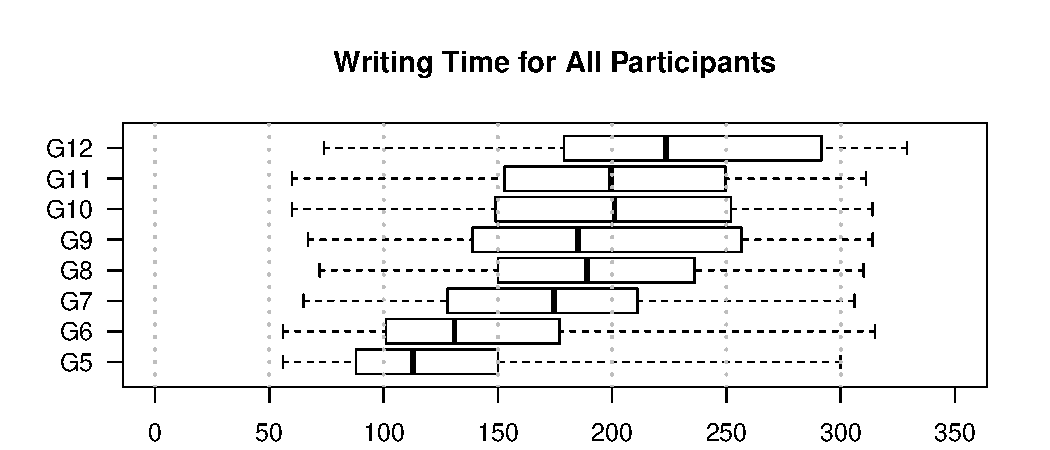
\includegraphics[width=\maxwidth]{figure/minimal-boxplots-minutes1-1} 

}



\end{knitrout}

\begin{knitrout}
\definecolor{shadecolor}{rgb}{0.969, 0.969, 0.969}\color{fgcolor}

{\centering 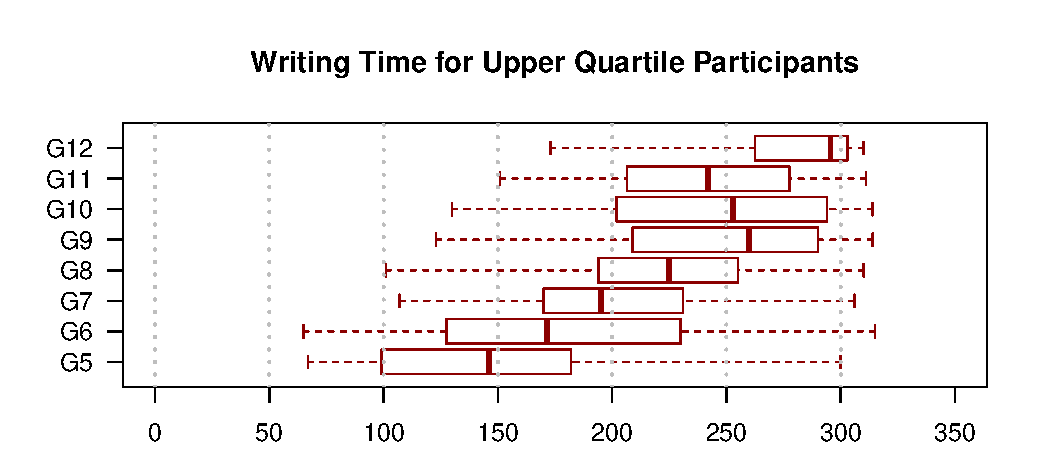
\includegraphics[width=\maxwidth]{figure/minimal-boxplots-minutes2-1} 

}



\end{knitrout}


\section{Dati par atsevišķajiem uzdevumiem}

\subsection{Vidējais vērtējums}

Ikviena uzdevuma vērtējums ir skaitlis no 0 līdz 10. Šajā tabulā apkopoti visu uzdevumu vidējie vērtējumi katrā no klašu grupām. Vidējo vērtējumu uzdevumam $X = \{ x_i \}$ aprēķina pēc formulas: 

\[ E(X) = \frac{\sum_{i=1}^{n}{x_i}}{n}, \]

\noindent
kur $x_i$ ir $i$-tā skolēna vērtējums par uzdevumu $X$, bet $n$ ir visu attiecīgās klases darbu skaits: $n = \left| X \right|$.

% Vidējais rezultāts pa uzdevumiem
\begin{knitrout}
\definecolor{shadecolor}{rgb}{0.969, 0.969, 0.969}\color{fgcolor}
\begin{tabular}{l|l|l|l|l|l}
\hline
  & Uzd1 & Uzd2 & Uzd3 & Uzd4 & Uzd5\\
\hline
G5 & 6.70 & 4.72 & 4.21 & 5.25 & 3.06\\
\hline
G6 & 6.35 & 4.41 & 4.02 & 2.96 & 7.27\\
\hline
G7 & 3.52 & 3.98 & 4.98 & 2.77 & 3.89\\
\hline
G8 & 4.44 & 4.91 & 3.70 & 5.32 & 5.41\\
\hline
G9 & 6.64 & 5.00 & 2.29 & 3.72 & 3.79\\
\hline
G10 & 4.53 & 6.12 & 2.71 & 5.31 & 2.09\\
\hline
G11 & 4.23 & 3.20 & 3.08 & 1.75 & 3.88\\
\hline
G12 & 7.09 & 3.61 & 5.38 & 4.17 & 2.57\\
\hline
\end{tabular}


\end{knitrout}

\noindent
Viszemākais un visaugstākais vidējais vērtējums ir attiecīgi 11.\ klases 4.\ uzdevumam (1.75) un 12.\ klases 1.\ uzdevumam (7.09).

\begin{uzdevums}[11.4]
Doti 99 naturāli skaitļi. Zināms, ka nav tāda skaitļa, ar ko dalītos visi šie skaitļi, un ka jebkuru 50 skaitļu reizinājums dalās ar atlikušo 49 skaitļu reizinājumu. Pierādīt, ka visu 99 skaitļu reizinājums ir naturāla skaitļa kvadrāts. 
\end{uzdevums}


\begin{uzdevums}[12.1]
Atrisināt nevienādību $9^x - 2 \cdot 3^x - 3 \leq 0$.
\end{uzdevums}






\subsection{Šenona entropija}

Entropiju uzdevuma $X$ vērtējumiem aprēķina pēc formulas:

\[ H(X) = - \sum_{i = 0}^{10}{p_i}\cdot \log_2{p_i}, \]

\noindent
kur $p_i = \frac{\left|\{ x \in X | x = i \}\right|}{\left| X \right|}$ ir varbūtība saņemt par uzdevumu $X$ vērtējumu $i$ (piemēram $p_0$ - vērtējumu "0 punkti" vai "uzdevums nav risināts" dalījums ar visu attiecīgās klases darbu skaitu). Ja kāds no vērtējumiem $i$ par attiecīgo uzdevumu nav sastopams, tad attiecīgo saskaitāmo entropijas formulā izlaiž.

Augsta entropija nozīmē augstu nenoteiktību. Ja visi vērtējumi par attiecīgo uzdevumu būtu vienādi, tad entropija ir 0. Ja visi vērtējumi no 0 līdz 11 ir vienādi bieži sastopami, tad entropija ir $\log2(11) \approx 3.46$. Pārāk zema entropija (piemēram tuvu 1 vai mazāka) nozīmē to, ka pats uzdevums vai tā vērtēšanas sistēma nav bijuši pārāk noderīgi olimpiādes dalībnieku punktu skaita diferencēšanai, jo pārāk daudzi vērtējumi ir vienādi.

\begin{knitrout}
\definecolor{shadecolor}{rgb}{0.969, 0.969, 0.969}\color{fgcolor}
\begin{tabular}{l|l|l|l|l|l}
\hline
  & Uzd1 & Uzd2 & Uzd3 & Uzd4 & Uzd5\\
\hline
G5 & 3.12 & 3.08 & 2.98 & 2.92 & 2.31\\
\hline
G6 & 3.11 & 2.92 & 2.74 & 2.16 & 2.12\\
\hline
G7 & 2.89 & 2.83 & 3.06 & 2.05 & 1.56\\
\hline
G8 & 2.79 & 3.34 & 2.42 & 3.02 & 2.82\\
\hline
G9 & 3.06 & 2.99 & 1.78 & 2.87 & 2.86\\
\hline
G10 & 2.64 & 1.60 & 1.79 & 3.26 & 0.80\\
\hline
G11 & 2.88 & 2.04 & 2.53 & 1.58 & 2.59\\
\hline
G12 & 2.83 & 2.29 & 3.30 & 1.61 & 1.79\\
\hline
\end{tabular}


\end{knitrout}


Viszemākā entropija ir bijusi 10.\ klases 5.\ uzdevuma vērtējumiem (0.80). Šie vērtējumi ir sekojoši (0 punkti - 252 darbos; 1 punkts - 10 darbos, 2 punkti - 4 darbos, 3 punkti - 1 darbā, 5 punkti - 1 darbā, 10 punkti - 4 darbos). 

\begin{uzdevums}[10.5]
Uz taisnstūra $ABCD$ diagonāles $BD$ iespējams atrast iekšēju punktu $P$ tā, ka
$\angle PAB = \angle PCB$. Pierādīt, ka $ABCD$ ir kvadrāts!
\end{uzdevums}






\subsection{Uzdevuma korelācija ar pārējo vērtējumu summu}

Izvēļu testu ({\em multiple choice exams}) analīzē bieži izmanto {\em biseriālo korelācijas koeficientu} --- kāda ir korelācija starp eksāmena kopīgo rezultātu un atbildēm (pareizas/nepareizas) uz konkrēto uzdevuma jautājumu. Ar šo skaitlisko kritēriju var atrast tos testu jautājumus, kuri varētu būt mulsinoši formulēti vai arī nemēra tās pašas prasmes, ko citi šī paša testa uzdevumi. 

Protams, olimpiāde nav izvēļu tests (un par katru no jautājumiem ir vairāk vērtējumu nekā tikai 0 vai 1). Tomēr arī šajā gadījumā korelācija var noderēt. Ja uzskatām, ka olimpiāde kopumā mēra noteikta veida matemātiskas prasmes, tad par katru uzdevumu var uzdot jautājumu: Cik labi šis uzdevums palīdz mērīt to pašu, ko olimpiādes uzdevumu komplekts kopumā? Ja konkrētais uzdevums labi ``iederas'' starp citiem, tad korelācija būs augsta, ja tas mēra kādas stipri atšķirīgas prasmes nekā citi tās pašas klases uzdevumi, tad korelācija būs mazāka. Korelāciju rēķina pēc šādas formulas:

\[ \mbox{cor}(X,Y) = \frac{\sum_{i=1}^{n}{x_i y_i} - n \cdot E(X) \cdot E(Y)}{\sqrt{\sum_{i=1}^{n}{x_i^2} - n \cdot E(X)^2} 
\cdot \sqrt{\sum_{i=1}^{n}{y_i^2} - n \cdot E(Y)^2}}, \]

\noindent
kur $x_i$ ir $i$-tā dalībnieka vērtējums par uzdevumu $X$, $y_i$ ir vērtējumu summa par visiem 4 atlikušajiem uzdevumiem, $n$ --- darbu skaits attiecīgajā klasē, $E(X)$ apzīmē $x_i$ aritmētisko vidējo.

Korelācijas koeficients vienmēr ir intervālā $[-1,1]$. Teorētiski varētu gadīties arī negatīva korelācija, t.i. tāds uzdevums, kuru veiksmīgākie olimpiādes dalībnieki risināja sliktāk nekā mazāk veiksmīgie. Tad paša uzdevuma vai vērtēšanas sistēmas korektums radītu nopietnas šaubas. Olimpiāžu praksē tomēr negatīvas korelācijas nav vērojamas. Salīdzinoši zemas uzdevuma vērtējuma korelācijas ar citiem uzdevumiem ļauj atrast tos uzdevumus, kuru tēma vai vērtēšanas kritēriji ir būtiski atšķīrušies no citiem uzdevumiem tajā pašā klases 5 uzdevumu komplektā.

\begin{knitrout}
\definecolor{shadecolor}{rgb}{0.969, 0.969, 0.969}\color{fgcolor}
\begin{tabular}{l|l|l|l|l|l}
\hline
  & Uzd1 & Uzd2 & Uzd3 & Uzd4 & Uzd5\\
\hline
G5 & 0.40 & 0.32 & 0.43 & 0.35 & 0.34\\
\hline
G6 & 0.33 & 0.22 & 0.25 & 0.26 & 0.18\\
\hline
G7 & 0.27 & 0.22 & 0.19 & 0.26 & 0.26\\
\hline
G8 & 0.38 & 0.33 & 0.40 & 0.32 & 0.24\\
\hline
G9 & 0.34 & 0.26 & 0.27 & 0.26 & 0.28\\
\hline
G10 & 0.31 & 0.13 & 0.16 & 0.30 & 0.14\\
\hline
G11 & 0.40 & 0.24 & 0.37 & 0.33 & 0.36\\
\hline
G12 & 0.18 & 0.14 & 0.16 & 0.05 & 0.31\\
\hline
\end{tabular}


\end{knitrout}

Mazākās korelācijas ar citiem tās pašas klases uzdevumiem ir 10.\ klases 2.\ uzdevumam (0.13) un 12.\ klases 4.\ uzdevumam (0.05). Šos uzdevumus varētu uzskatīt par ``visjocīgākajiem'', kas prasīja prasmes, kas stipri atšķiras no citos uzdevumos nepieciešamajām. 

\begin{uzdevums}[10.2]
Dotas divas paralēlas taisnes. Uz vienas no tām atzīmēti 14 zaļi punkti, uz otras -- 14 sarkani punkti. Kādu lielāko skaitu nogriežņu, kuriem viens galapunkts ir zaļš, bet otrs -- sarkans, var novilkt tā, lai tie nekrustotos? Saka, ka nogriežņi krustojas, ja tiem ir kopīgs iekšējais punkts, t.i., ja tiem ir kopīgs tikai galapunkts, tie nekrustojas.
\end{uzdevums}


\begin{uzdevums}[12.4]
Vai kvadrātu ar malas garumu 10 var noklāt ar 25 ``krustiņiem'' (skat. zīm.), kuri sastāv no 5 kvadrātiem ar malas garumu 1? ``Krustiņi'' drīkst pārklāties, kā arī iziet ārpus dotā kvadrāta malām.\\

\includegraphics[width=14mm]{pentomino-x.png}
\end{uzdevums}







\subsection{Vērtējumu atšķirības zēniem un meitenēm}

Vērtējumu atšķirību konkrētas klases uzdevumam $X$ aprēķina kā divu vidējo vērtību starpību: 

\[ \Delta_{\mbox{gender}}(X) = E\left(X_{\mbox{male}}\right) - E\left(X_{\mbox{female}}\right), \]

\noindent
kur $X_{\mbox{male}}$ ir visi attiecīgās klases zēnu vērtējumi un  $X_{\mbox{female}}$ ir attiecīgās klases meiteņu vērtējumi, un $E(X)$ - skaitļu virknes $X$ aritmētiskais vidējais.

\begin{knitrout}
\definecolor{shadecolor}{rgb}{0.969, 0.969, 0.969}\color{fgcolor}
\begin{tabular}{l|l|l|l|l|l}
\hline
  & Uzd1 & Uzd2 & Uzd3 & Uzd4 & Uzd5\\
\hline
G5 & 0.80 & 0.08 & 0.19 & -0.63 & 0.12\\
\hline
G6 & 0.86 & -0.28 & 0.60 & 0.12 & 1.88\\
\hline
G7 & -0.08 & -0.00 & 0.97 & -0.41 & -0.26\\
\hline
G8 & 0.94 & 0.27 & -0.19 & 0.07 & 0.25\\
\hline
G9 & 0.67 & -0.36 & 0.08 & 0.93 & -0.38\\
\hline
G10 & 0.20 & -0.13 & -0.02 & 0.07 & 0.01\\
\hline
G11 & 0.16 & 0.93 & -0.21 & -0.03 & -0.01\\
\hline
G12 & -0.34 & -0.50 & -0.39 & -0.03 & -0.50\\
\hline
\end{tabular}


\end{knitrout}

Katram no uzdevumiem atrasta zēnu un meiteņu vidējo vērtējumu starpība. Pozitīvs skaitlis nozīmē to, ka zēnu vērtējums bija augstāks, negatīvs skaitlis --- to, ka meiteņu vērtējums bija augstāks. Vislielākās priekšrocības zēniem bija risinot 6.\ klases 5.\ uzdevumu (1.88 punktu pārsvars); savukārt meitenēm --- risinot 5.\ klases 4.\ uzdevumu (0.63 punktu pārsvars). Neparasti, ka abi šie uzdevumi ir par līdzīgu tēmu --- rūtiņu laukuma aizpildīšanu ar figūriņām. Šī pārskata mērķis nav noskaidrot, vai atšķirības ir statistiski būtiskas. Varbūt dzimumu atšķirības radīja ne vien pats uzdevums, bet arī noteikta veida vērtēšanas kritēriji. Diez vai to ir iespējams precīzi noskaidrot, ja pēc olimpiādes darbu labošanas pagājis vairāk nekā 1 gads. 

\begin{uzdevums}[6.5]
Rūtiņu kvadrātā $5 \times 5$ iekrāsot iespējami maz rūtiņu tā, lai atlikušajā daļā vairs nevarētu ievietot nevienu zīmējumā redzamo figūru (tā var būt gan pagriezta, gan apgāzta). Pamatot, ka iekrāsoto rūtiņu skaits ir mazākais iespējamais!\\
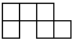
\includegraphics[width=20mm]{hexomino.png}
\end{uzdevums}


\begin{uzdevums}[5.4]
Kvadrāts sastāv no $8 \times 8$ vienādām kvadrātiskām rūtiņām. Tas sagriezts daļās tā, ka griezumi iet pa rūtiņu robežām. Kāds lielākais skaits daļu var būt tādas kā zīmējumā attēlotā figūra (figūras var būt pagrieztas jebkurā stāvoklī)?\\
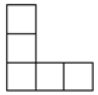
\includegraphics[width=14mm]{pentomino-v.png}
\end{uzdevums}



\end{document}
